\chapter{Working Principles of Germanium Detectors}

\section{Interaction of radiation with Matter}
\begin{figure}[htpb]
\centering
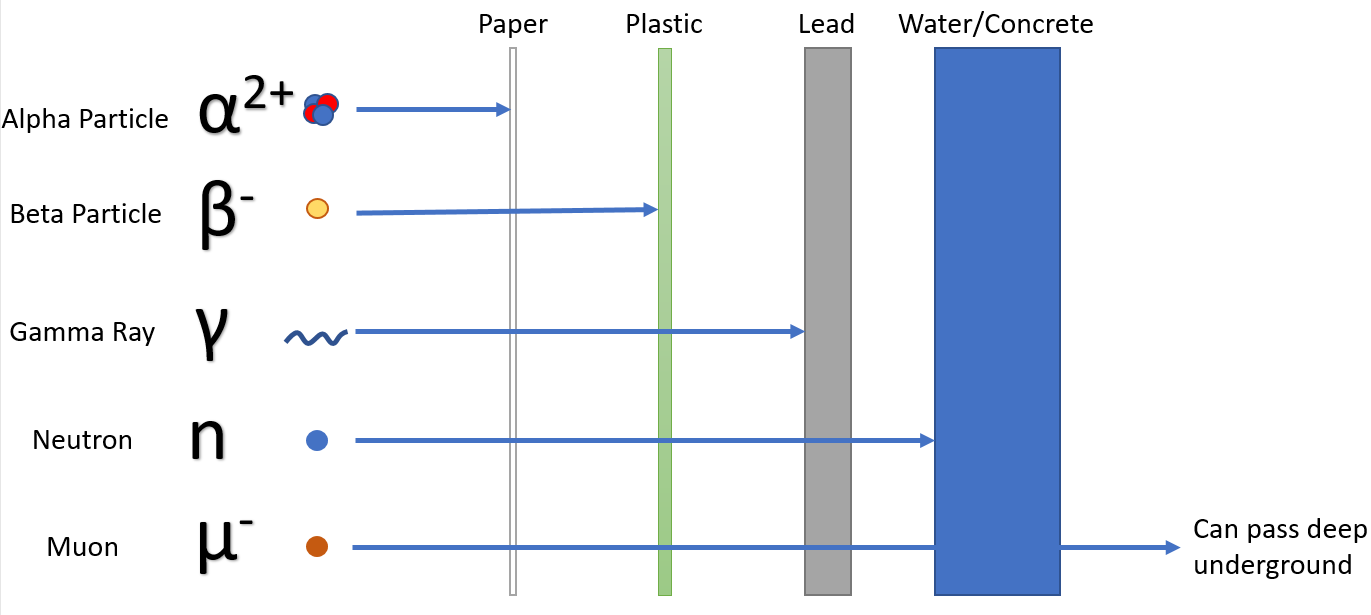
\includegraphics[width=0.8\textwidth]{penetration}
\caption{Various penetration capabilities of several types of radiation}
\label{fig:penetration}
\end{figure}

Different interactions
Photoelectric
Compton
Pair production

2.6 MeV highest natural radiation

Include chart with all three and effects at different energy

For alphas, worry about surface contamination but most is blocked by shielding

For Betas, blocked by cryostat. special use case, beryllium windows like SEM.

Neutrons no charge so must interact with nucleus, slowest are capture, can decay or change atom which creates gamma

elastic scattering, gives nuclear recoil

inelastic scattering gives nuclear recoil and can excite which gives gamma

Spallation blow up the atom to parts which gives off huge energy

Muon, negative charged, most come from cosmic ray, minimum ionization particle. creates a huge deposition of energy in very short time. can also spallate

Protons, can behave like a neutron or muon, can interact with EM field or nucleus- might not be needed.

\section{Spectroscopy}

understand the spectrum based on energy, compton shoulder, peaks, overall shape, etc Knolls book Ch10.F.2
energy resolution-random process for creation of electrons and holes 2.9 eV (average energy required to create electron hole pair) can also be caused by electron noise. some trapping of electrons and holes.
energy calibration,

\section{semiconducter diode detector}
Read all of chapter 11, skip section VI, Channeling
Read chapter 12
